\documentclass{article}

\usepackage{amsmath}
\usepackage{palatino}
\usepackage{tikz}

\newcommand{\diag}{\Delta}
\newcommand{\ccat}{\mathbf{C}}
\newcommand{\id}{\mathbf{id}}
\newcommand{\pow}{\mathcal{P}}
\newcommand{\fpow}{\mathbf{\mathcal{P}}}
\newcommand{\cset}{\mathbf{Set}}

\begin{document}

\begin{enumerate}
\item[2.1.4]
  We want to show that the definitions \emph{maplist}:
  \begin{align*}
    \emph{maplist}(f)([]) &= []
    \\ \emph{maplist}(f)([x]) &= [f x]
    \\ \emph{maplist}(f)(L * L') &= \emph{maplist}(f)(L) * \emph{maplist}(f)(L')
  \end{align*}
  and \emph{maplist'}
  \begin{align*}
    \emph{maplist'}(f)([]) &= []
    \\ \emph{maplist'}(f)([x] * L) &= [f x] * \emph{maplist'}(f)(L)
  \end{align*}
  are equivalent.
  This follows by the associativity of *.
  The second definition forces right associativity and the first allows any parenthesization.

\item[2.1.10.1]
  \begin{itemize}
  \item Example 2.1.5, the forgetful functor on monoids, satisfies the definition of a functor because it takes the identity homomorphism to the identity on the underlying set and the result of $F (f;g)$ for homomorphisms $f : (M,\cdot,e) \rightarrow (M',\cdot',e')$ and $g : (M',\cdot', e') \rightarrow (M'',\cdot'',e'')$ is $F(f); F(g)$ where $F(f) : M \rightarrow M'$ and $F(g) : M' \rightarrow M''$ are defined on the underlying sets. 
    Thus identities and composition are preserved.
  \item Example 2.1.6, the identity functor, trivially preserves identities and composition.
  \item Example 2.1.7, the right product functor, takes the identity arrow for an object $B$ to the product $(id_B, id_A)$, which is the identity arrow for the resulting pair, and maps compositions to the composition of product arrows $(f,id_A); (g,id_A)$, which is well-defined in the product category.
  \end{itemize}

\item[]
\item [2.1.10.2]
  We define the powerset operator $\pow : S \rightarrow 2^S$, as an endofunctor $\fpow$ on the category $\cset$.
  \begin{itemize}
  \item For objects $A \in \cset$, $\fpow(A)$ is the powerset of $A$, $\pow(A) \in \cset$.
  \item Identity arrows on sets $A$ are lifted to identity arrows on the corresponding powerset, $\pow(A)$.
    This the functor conserves identities.
  \item For morphisms $f : A \rightarrow B$, $\fpow(f) : \pow(A) \rightarrow \pow(B)$ is the result of applying $f$ to all sets $a \in \pow(A)$.
    Composition $g \circ f$ is then preserved because $f : A \rightarrow B$ maps to $\fpow(f) : \pow(A) \rightarrow \pow(B)$ and $g : B \rightarrow C$ maps to $\fpow(g) : \pow(B) \rightarrow \pow(C)$.
  \end{itemize}

  At first I wanted to define $\fpow(f)$ as extracting the highest-cardinality element $A$ from the set $\pow(A)$, applying $f(A)$, then taking $\pow(f(A))$.
  But if $A$ is the domain of $f$ then we can take $f(A')$ for any $A' \subseteq A$, so it's easier this way.
\item[]
\item[2.1.10.3] The functors between monoids considered as one-object categories are the structure-preserving maps between the two monoids.
  These are monoid homomorphisms.

\item[]
\item [2.1.10.4]
  Pierce defines the diagonal functor $\diag : \ccat \rightarrow \ccat \times \ccat$ on a category $\ccat$ as taking each $\ccat$-object $A$ to the object $(A,~A)$.
  
  The corresponding action of $\diag$ on arrows takes morphisms $f$ to the pair of morphism $(f,~f)$.
  Identities are preserved because $(\id_A,~\id_A)$ is the identity arrow for the object $(A,~A) \in \ccat \times \ccat$ and composition is similarly the composition of arrows applied pointwise in $\ccat \times \ccat$.

\item[]
\item [2.1.12]
  In the contravariant hom-functor for an object $B \in \ccat$, called $\ccat(-,B)$:
  \begin{itemize}
  \item Each object $A \in \ccat$ maps to $\ccat(A,B)$, the set of all arrows from $A$ to $B$.
  \item Each arrow $f : A \rightarrow C$ maps to the function $\ccat(f, B) : \ccat(C,B) \rightarrow \ccat(A,B)$ defined for a function $g : C \rightarrow B$ as $\ccat(f,B)(g) = g \circ f$.
  \end{itemize}

  This hom-functor combined with the covariant one combine to form a bifunctor where:
  \begin{itemize}
  \item Each pair of objects $A,B$ map to $\ccat(A,B)$, the set of all morphisms from $A$ to $B$.
  \item Each pair of arrows $f : C \rightarrow A,~g : B \rightarrow D$ define a functor $\ccat(f,g) : \ccat(A,B) \rightarrow \ccat(C,D)$
  \item An object, arrow pair or an arrow, object pair behave like the covariant and contravariant hom-functors, respectively.
  \end{itemize}
  The bifunctor arises because the following diagram commutes for functions $f : C \rightarrow A$ and $g : B \rightarrow D$.

  \begin{center}
    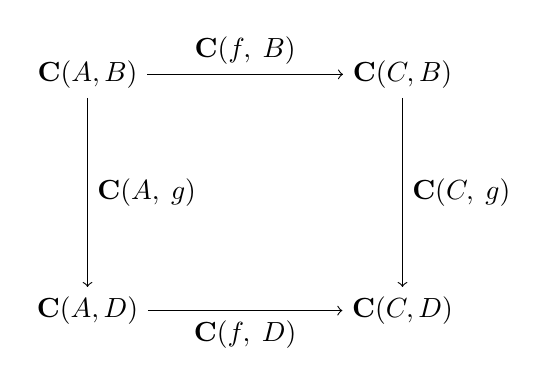
\begin{tikzpicture}
      \node (1) {$\ccat(A,B)$};
      \node[right of=1,xshift=3cm] (2) {$\ccat(C,B)$};
      \node[below of=1,yshift=-2cm] (3) {$\ccat(A,D)$};
      \node[below of=2,yshift=-2cm] (4) {$\ccat(C,D)$};

      \draw[->] (1) -- node[above] {$\ccat(f,~B)$} (2);
      \draw[->] (1) -- node[right] {$\ccat(A,~g)$} (3);
      \draw[->] (2) -- node[right] {$\ccat(C,~g)$} (4);
      \draw[->] (3) -- node[below] {$\ccat(f,~D)$} (4);
    \end{tikzpicture}
  \end{center}
  
\end{enumerate}

\end{document}
